\solution{
\paragraph{Experimental environment.}
All measurements were collected on one NVIDIA L4 (23,034 MiB)
using vLLM 0.10.2, CUDA 12.8, and PyTorch 2.8.0+cu128. Each checkpoint was loaded and measured
separately on the same GPU. Exact software and model revisions are recorded in
\texttt{results/serving\_metadata.json}.

\paragraph{Serving configuration.}
All checkpoints were loaded with on-the-fly FP8 weight quantization
(\texttt{--quantization fp8}) and an FP8 KV cache
(\texttt{--kv-cache-dtype fp8}). Tensor parallelism was one. We fixed the
maximum model length at 4096, GPU memory utilization at 0.90, the maximum
number of sequences at 64, and the maximum batched-token budget at 32768.
We performed one warm-up and then three recorded repetitions per condition.

\paragraph{Prefill-dominated workload.}
We swept exact tokenized input lengths
\[
L\in\{128,512,1024,2048,3072\},
\]
used eight simultaneous requests, and generated one output token per request.
For batch wall-clock time $t$, prefill throughput was
\[
T_{\mathrm{prefill}}=\frac{\sum_i L_i}{t}.
\]
Inputs were passed as token IDs, so the intended length was exact for every
checkpoint. Deterministically rotated natural-text token sequences prevented
prefix-cache reuse between requests.

\paragraph{Decode-dominated workload.}
We fixed each input at 32 tokens and forced exactly 256 output tokens by
ignoring EOS. We varied the number of parallel generations over
\[
C\in\{1,2,4,8,16,32,64\}.
\]
Aggregate decode throughput was
\[
T_{\mathrm{decode}}=\frac{\sum_i O_i}{t},
\]
where $O_i=256$ for every request.

\begin{figure}[t]
  \centering
  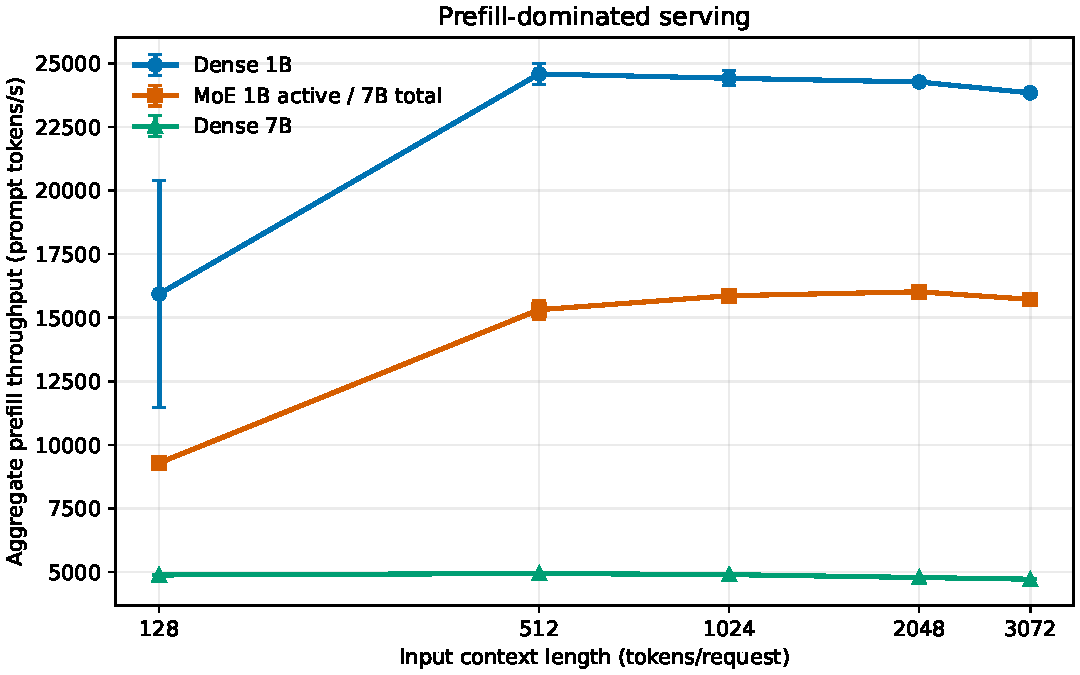
\includegraphics[width=0.86\linewidth]{figures/prefill_throughput.pdf}
  \caption{Mean aggregate prefill throughput versus input context length.
  Error bars show one sample standard deviation across three repetitions.}
  \label{fig:prefill-throughput}
\end{figure}

\begin{figure}[t]
  \centering
  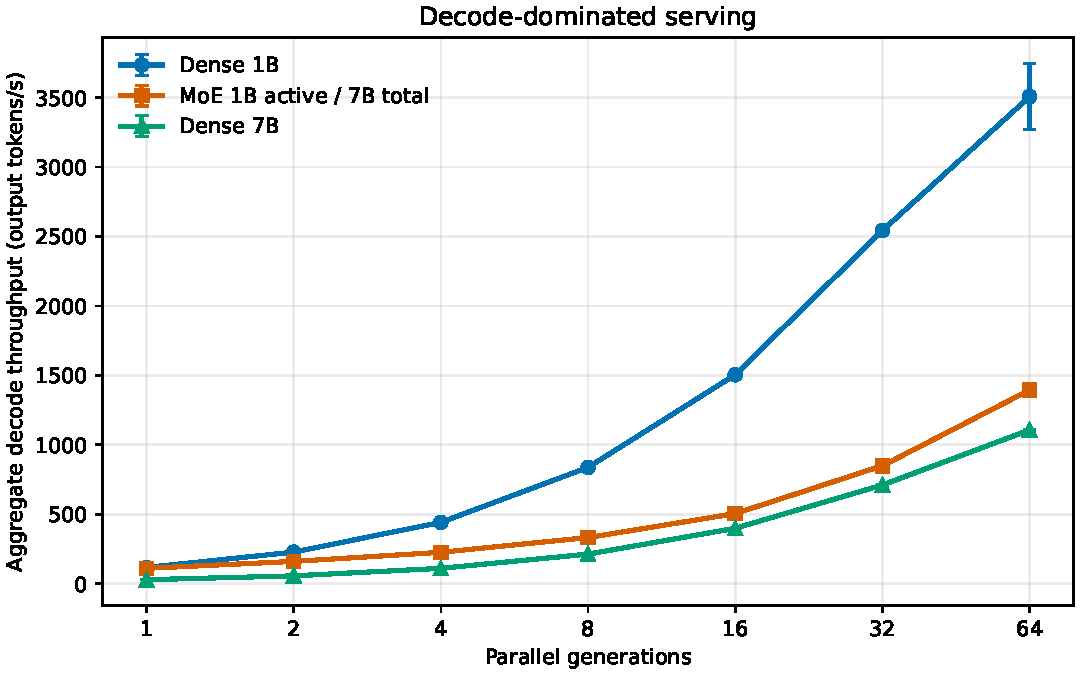
\includegraphics[width=0.86\linewidth]{figures/decode_throughput.pdf}
  \caption{Mean aggregate decode throughput versus parallel generations.
  Error bars show one sample standard deviation across three repetitions.}
  \label{fig:decode-throughput}
\end{figure}

\paragraph{Results and interpretation.}
OLMoE beat the 7B dense model at every measured point, but did not overtake
the 1B dense model. Its prefill advantage over the 7B model grew from about
$1.9\times$ at 128 tokens to $3.3\times$ at 3072 tokens. During decode, the
advantage narrowed from $3.9\times$ at one generation to $1.26\times$ at 64.
Only about 1B expert parameters are active per token, so OLMoE's arithmetic
cost is closer to the small dense model. However, all 7B parameters remain in
memory, and concurrent requests touch a wider set of experts. Expert-weight
traffic and routing overhead therefore make its high-concurrency behavior
closer to the large dense model. These mechanisms are consistent with the
OLMoE architecture described by \citet{muennighoff2025olmoe}.

\paragraph{Artifacts.}
The full experiment is implemented in
\texttt{scripts/benchmark\_serving.py}. Raw per-repetition measurements are in
\texttt{results/serving\_raw.csv}; plotting and aggregation are implemented in
\texttt{scripts/plot\_serving\_results.py}. A generated numerical summary can
be included with \texttt{\textbackslash input\{results/summary\_table.tex\}}.
}
